\section{Svolgimento dello stage}
	\subsection{}
		\begin{frame}{Metodologia di lavoro}
			\begin{figure}
				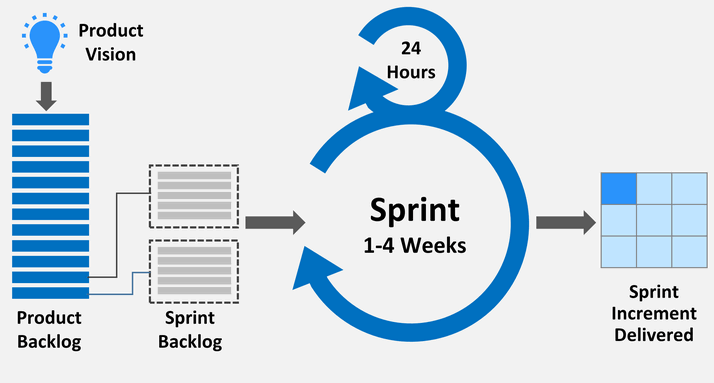
\includegraphics[width=0.99\textwidth]{capitolo_3/immagini/scrum.png}
			\end{figure}
		\end{frame}
	\subsection{}
		\begin{frame}{Analisi dei requisiti}
			\emph{Obbligatori}
				\begin{itemize}
							\item Creazione e gestione canale
							\item Implementazione utenti
							\item Sistema di permessi
				\end{itemize}
			\emph{Opzionali}
				\begin{itemize}
						\item Integrazione interfaccia grafica
						\item Unione con applicazione Android
				\end{itemize}
			\end{frame}
	\subsection{Sviluppo Server Java}
	\begin{frame}{Eclipse Vert.x}
		\begin{minipage}{0.5\textwidth}
			\emph{Vantaggi}
						\begin{itemize}
							\item alta scalabilità
							\item poliglotta
							\item documentazione
						\end{itemize}
			\emph{Costrutti fondamentali}
				\begin{itemize}
					\item Event Loop
					\item Event Bus
					\item Verticle
				\end{itemize}
			\end{minipage}
			\begin{minipage}{0.3\textwidth}
					\begin{figure}
						
\includegraphics[width=1.2\textwidth]{capitolo_3/immagini/Vertx.png}
					\end{figure}
				\end{minipage}
			\end{frame}
	\subsection{Sviluppo Server Java}
		\begin{frame}{Progettazione}
			\begin{minipage}{0.6\textwidth}
				\emph{Canale di comunicazione}
					\begin{itemize}
						\item Creazione ed eliminazione
						\item Invio e ricezione di \emph{messaggi}
						\item Aggiunta e rimozione \emph{utenti}
					\end{itemize}
			\end{minipage}
			\begin{minipage}{0.3\textwidth}
				\begin{figure}
					
\includegraphics[width=0.7\textwidth]{capitolo_3/immagini/comunicazione.png}
				\end{figure}
			\end{minipage}
			\begin{minipage}{0.6\textwidth}
				\emph{Utenti}
					\begin{itemize}
						\item Amministratore
						\item Utente Base
					\end{itemize}
			\end{minipage}
			\begin{minipage}{0.3\textwidth}
				\begin{figure}
					
\includegraphics[width=0.7\textwidth]{capitolo_3/immagini/utenti.jpg}
				\end{figure}
			\end{minipage}
			\begin{minipage}{0.6\textwidth}
				\emph{Sistema di autorizzazione}
				\begin{itemize}
					\item Lato Utente (richiesta)
					\item Lato Amministratore (autorizzazione/rimozione)
				\end{itemize}
			\end{minipage}
			\begin{minipage}{0.3\textwidth}
				\begin{figure}
					
\includegraphics[width=0.7\textwidth]{capitolo_3/immagini/autorize.jpg}
				\end{figure}
			\end{minipage}
		\end{frame}
	\subsection{Sviluppo Server Java}
		\begin{frame}{Implementazione}
			\begin{minipage}{0.4\textwidth}
				\emph{Canale di comunicazione}
					\begin{itemize}
						\item Messaggi $\rightarrow$ JSON
						\item EventBus $\rightarrow$ Vert.x
					\end{itemize}
			\end{minipage}
			\begin{minipage}{0.4\textwidth}
				\begin{figure}
					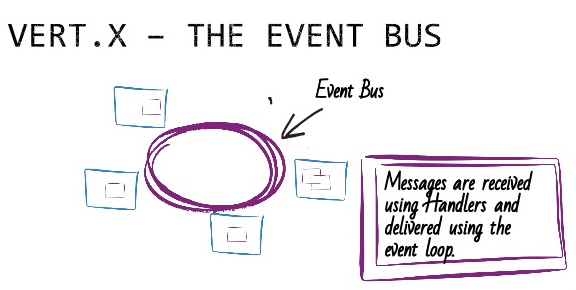
\includegraphics[width=1.6\textwidth]{capitolo_3/immagini/eventbus.jpg}
				\end{figure}
			\end{minipage}
			\begin{minipage}{0.3\textwidth}
				\emph{Utenti}
					\begin{itemize}
						\item User (interfaccia)
						\item UserBase
						\item Admin
					\end{itemize}
			\end{minipage}
			\begin{minipage}{0.5\textwidth}
				\emph{Sistema di autorizzazione}
				\begin{itemize}
					\item Utente $\rightarrow$ request()
					\item Amministratore $\rightarrow$ authorize(UserBase[])
				\end{itemize}
			\end{minipage}
		\end{frame}
	\subsection{}
		\begin{frame}{Interfaccia grafica}
			\begin{minipage}{0.4\textwidth}
				\begin{block}{Moduli utilizzati}
					\begin{itemize}
						\item Vert.x HTTPServer
						\item Vert.x WebSocket
					\end{itemize}
				\end{block}
			\end{minipage}
			\begin{minipage}{0.5\textwidth}
				\begin{figure}
					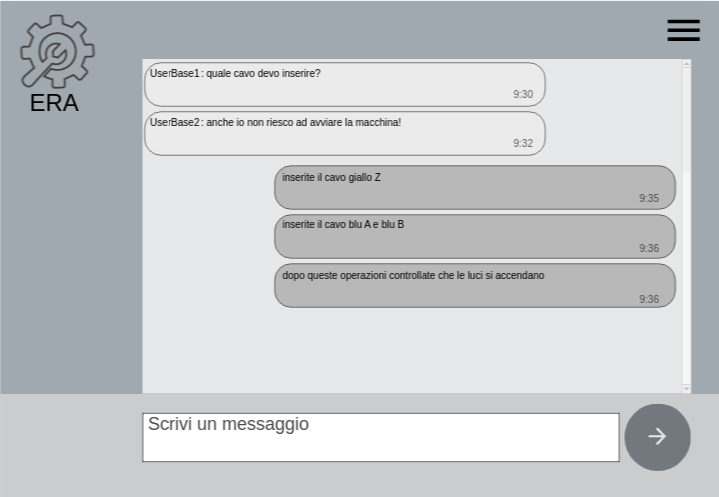
\includegraphics[width=1.2\textwidth]{capitolo_3/immagini/chat.png}
				\end{figure}
			\end{minipage}
			\begin{minipage}{0.3\textwidth}
				\begin{figure}
					
\includegraphics[width=0.5\textwidth]{capitolo_3/immagini/js.png}
				\end{figure}
			\end{minipage}
			\begin{minipage}{0.4\textwidth}
				\begin{block}{Funzioni}
					\begin{itemize}
						\item invio e ricezione
						\item autorizzazione
					\end{itemize}
				\end{block}
			\end{minipage}
		\end{frame}
